\subsection{Solución Propuesta}

La solución que se propone ( como se ha mencionado anteriormente ), es el desarrollo de un sistema de gestión descentralizado de la financiación de proyectos, usando los beneficios de la tecnología blockchain.

\bigskip

La plataforma a desarrollar se regirá mediante un mecanismo de gestión autónomo para evitar que un administrador u otra entidad pueda malversar los fondos de la plataforma.

\bigskip

La comunidad decidirá qué proyectos se aprobarán y cuáles no. Los proyectos pasarán por un proceso de votación antes de ser aceptados donde cada usuario podrá votar una única vez en un proyecto, para verificar la integridad de la idea, la veracidad, la viabilidad, y para detectar cualquier incongruencia en la descripción, los hitos propuestos y los fondos requeridos para su desarrollo.

\bigskip

En concreto, la propuesta de proyecto, tendrá ( entre otros ), titulo, descripción, naturaleza / tipo, cantidad de fondos necesarios para su formalización, tiempo total para su desarrollo, lista de hitos, y por cada hito: titulo, descripción y \% del tiempo total del desarrollo asignado para dicho hito.

\bigskip

Esta fase tendrá una duración limite de 30 días desde la propuesta del proyecto, y los votos positivos necesarios para aprobar la propuesta deben ser igual o superior al 85\% de los votos presentados, en caso de no alcanzar dicho umbral, se denegará la propuesta.

\bigskip

Se permitirá a los usuarios comentar los proyectos propuestos, lo que fomentará la interacción en la comunidad al compartir ideas, debatir sobre cada proyecto y comunicarse con el proponente. De este modo, se mantendrá una dinámica activa y se compartirá el progreso de cada proyecto.

\bigskip

Una vez aprobado por la comunidad, empieza la fase de financiación. Los usuarios pueden invertir en el proyecto durante un periodo de 30 días y una vez se recauden los fondos necesarios empezará la fase de desarrollo, dónde los fondos se desbloquearán de forma secuencial conforme se vayan cumpliendo y validando los hitos del desarrollo. En caso de no alcanzar la cuota necesaria definida en la propuesta en estos 30 días, la propuesta se denegará, y los fondos recaudados se reembolsarán a cada inversor.

\bigskip

El proponente podrá solicitar la revisión de cada hito para su validación. Los hitos serán validados por la comunidad, en concreto usuarios \quotes{peritos} con cierta especialización en la naturaleza del proyecto. Esta especialización será validada mediante un modelo de verificación de credenciales\cite{w3c}. Estos se encargarán de validar que los hitos se han alcanzado correctamente. 

\bigskip

El hito se dará por cumplido cuando por votación, la mayoría absoluta de los votos recibidos por los peritos aprueban el hito, en caso contrario, el perito discrepante deberá adjuntar el motivo de su negación. Si el hito no se cumple, se le proporcionará al proponente el motivo de la denegación ( motivos de los votos negativos ), y un tiempo limitante de 10 días para poder solventar el hito, al cabo de este tiempo el proponente podrá nuevamente volver a solicitar la validación del hito.

\bigskip

En un último acontecimiento en el cual el proyecto muestra claras señales de estancamiento, como por ejemplo: haber excedido el plazo para la solicitud de revisión del avance de los hitos en un plazo estimable al doble del tiempo asociado a cada hito, la propuesta del proyecto se cancelará automáticamente, y el resto de los fondos asignados al los hitos sin alcanzar se reembolsará a los inversores.

\bigskip

Para cumplir con esta solución, es esencial garantizar la trazabilidad y el control de los fondos y activos de la plataforma. Además, para evitar que el proponente o un miembro malintencionado de la comunidad pueda eliminar o cambiar un proyecto durante su proceso los datos del proyecto deben ser inmutables.

\begin{figure}[H]
        \centering
        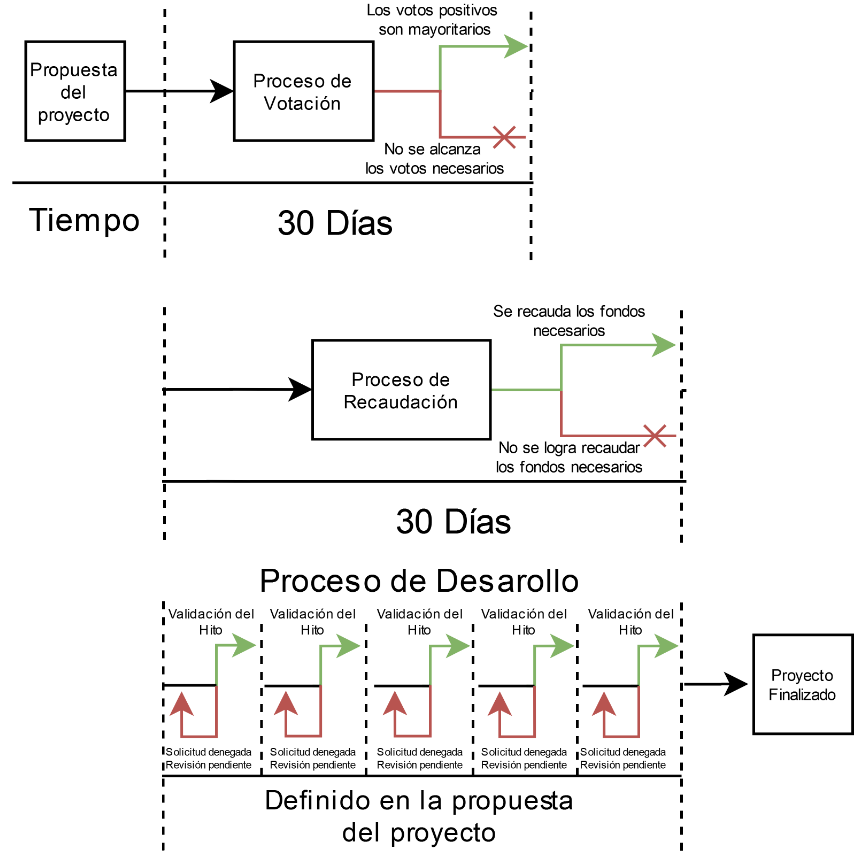
\includegraphics[width=0.9\textwidth]{img/diagramas/proceso_vertical.png}
        \caption{Representación del proceso de inversión.}
        \label{fig:configApi}
\end{figure}

El uso de una blockchain para este trabajo es una aportación perfecta para desarrollar el trabajo, ya que a través de la trazabilidad que nos proporciona podremos ver en que se gastan los activos y además tener un control sobre estos, y un transparencia total con los usuarios. 

\bigskip

De esta forma pudiendo así implementar una solución la cual desbloqueará parte de lo recaudado a medida que se van completando ciertos hitos asociados al desarrollo del proyecto.

\newpage

\subsection{Abstracción del problema aborado}

La solución propuesta, un sistema de gestión descentralizado de la financiación de proyectos basado en la tecnología blockchain, puede ser aplicable a una serie de contextos más allá de las plataformas de crowdfunding.

\bigskip

Estos pueden incluir la gestión de proyectos en organizaciones, la trazabilidad de la financiación de proyectos en instituciones financieras y la verificación del cumplimiento de las regulaciones en el transporte de mercancías, etc.

\bigskip

El conjunto de problemas presentado puede categorizarse como "Gestión y trazabilidad de proyectos financiados colectivamente". Dichos problemas son intrínsecos a cualquier plataforma o sistema que maneje la financiación y el desarrollo de proyectos. Los problemas pueden subdividirse en los siguientes aspectos clave:

\bigskip

\begin{itemize}
    \item \textbf{Autenticidad y Veracidad:} Corresponde a las dificultades para verificar la autenticidad de un proyecto y la honestidad de los creadores del mismo. Incluye problemas como fraudes, estafas y malversación de fondos, donde los creadores del proyecto pueden engañar a los inversores acerca de la naturaleza, el resultado y/o la causa solicitada del proyecto.
    
    \item \textbf{Gestión de la Financiación:} Se refiere a la complejidad de rastrear y manejar adecuadamente los fondos recaudados. Entra en juego cuando se enfrentan problemas de malversación de fondos, lavado de dinero y falta de transparencia en la distribución y uso de los fondos recaudados.
    
    \item \textbf{Validación del Progreso:} Se refiere a las dificultades para verificar el cumplimiento de los hitos propuestos y para validar el progreso del proyecto. Los creadores del proyecto pueden engañar a los inversores y otros interesados acerca del progreso real y los logros del proyecto.
    
    \item \textbf{Participación y Decisión:} Se refiere a las dificultades para permitir y manejar la participación de la comunidad en la toma de decisiones, la validación del proyecto y la revisión de los hitos. Situaciones donde la comunidad se siente excluida del proceso de toma de decisiones y la falta de transparencia y control pueden provocar una disminución de la confianza y la participación.
    
\end{itemize}